\section{GPT Overview}
\begin{frame}\frametitle{What is GPT?}
  A standard developed by Intel in the late '90s for the layout of the partition table on a physical hard disk.\newline

  It overcomes major limitations of MBRs and today forms part of the \textbf{UEFI} standard.
\end{frame}

\subsection{Benefits of GPT}
\begin{frame}\frametitle{Benefits of GPT}
  So, what's the big deal about GPT?
  \begin{itemize}
  \item Forget extended or logical DOS-like partitions. GPT can handle at least 128 partitions.
  \item 64-bit sectors gives us $2^{64}$ available sectors, or 9.4 Zb partitions (with 512 bytes).
  \item 32-bit CRC checksums to ensure data integrity.
  \item Redundant data structures help protect against disk errors.
  \end{itemize}
\end{frame}

\subsection{Drawbacks of GPT}
\begin{frame}\frametitle{Drawbacks of GPT}
  There's no such thing as a free lunch:
  \begin{itemize}
    \item s
  \end{itemize}
\end{frame}

\begin{frame}
  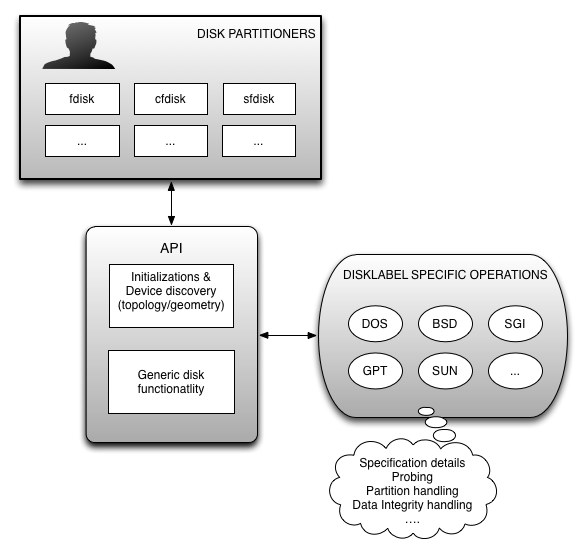
\includegraphics[scale=0.35]{img/fdisk-arch.png}
\end{frame}
